\chapter{VM Provisioning of Scientific Workflows in a Single Site Cloud} \label{MOVMPSWC}

A Cloud provide diverse computing resources and appear as appropriate infrastructures for executing Scientific Workflows (SWfs).
However, the problem of how to provision Virtual Machines (VMs) is critical for SWf execution.
In addition, since SWf execution takes much time and money, it is important to achieve multi-objectives, \textit{i.e.} reducing both execution time and monetary cost.
In this chapter, we address a problem of how to provision VMs to execute a SWf in a multisite cloud, while reducing execution time and monetary costs.
The solution consists of a multi-objective cost model including execution time and monetary costs and a Single Site VM Provisioning approach (SSVP).
We present an experimental evaluation, based on the execution of the SciEvol SWf in Microsoft Azure cloud. This chapter is based on \cite{Liu16}.

Section \ref{sec:PMoO} propose our multi-objective cost model. 
Then, Section \ref{sec:PVMD} describes our SSVP algorithm including the SciEvol SWf use case.
Section \ref{sec:PVal} presents our experimental evaluation in Microsoft Azure cloud \cite{Azure}.
The results reveal that our cost model is accurate and that SSVP can generate better VM provisioning plans compared with an existing approach.

\section{Motivations and Overview}

SWfs are used to model large-scale \textit{in silico} scientific experiments to process big amounts of data. In order to process big data, the execution of SWfs generally takes much time. As a result, it is important to use parallelism techniques to execute SWfs within a reasonable time. Some SWf Management Systems (SWfMSs) with parallelism techniques already exist, \textit{e.g.} Pegasus \cite{Deelman2005,Deelman2014}, Swift \cite{Zhao2007}, Chiron \cite{Ogasawara2013}, which can take advantage of clusters, grids, and clouds to execute SWfs.

Since a cloud offers diverse resources, virtually infinite computing and storage resources, it becomes an interesting infrastructure for SWf execution. 
For instance, Infrastr-ucture-as-a-Service, \textit{i.e.} IaaS, providers offer VMs to the general public, including scientists, through the Internet \cite{Gonzalez09}.
Diverse types of VMs are available.  The VM type determines some parameters such as the number of virtual CPUs, the size of memory and the default storage size of hard disk.
The VMs can be used to create a cluster in the cloud. 

However, the problem of choosing the number and the type of VMs remains a critical problem for SWf execution in the cloud since the estimation involves various parameters, such as VM types, different SWfs \cite{Coutinho2014}. 
Although some existing VM provisioning solutions exist, some \cite{Emeakaroha13} focus on a single objective and some generate provisioning plans without consideration of the workload of SWfs \cite{Shen11,Coutinho2014} or just simulates SWf execution to validate the approach \cite{Xu12}.
SciDim \cite{Oliveira13} is proposed to generate a provisioning plan based on a heuristic, \textit{i.e.} genetic algorithm. However, it depends on the provenance data and needs to dynamically modify the provisioning plans, which are not supported by most SWfMSs.
Coutinho \textit{et al.} \cite{Coutinho2014} propose a GraspCC algorithm to generate a provisioning plan for SWf execution. However, GraspCC relies on the strong assumption that the entire workload of SWfs can be executed in parallel. Furthermore, it cannot reuse existing started VMs and its cost model is too simple, \textit{e.g.} does not consider the cost of starting VMs, which may be high with many VMs to provision.
As a result, the real execution time of two SWfs (SciEvol and SciPhylomics \cite{Oliveira2013}) in Amazon EC$2$ \cite{AmazonCloud} is two times the estimated time.
In addition, some cost models \cite{Oliveira2012}\cite{Sardina2010} for SWf scheduling cannot be used for generating a proper number of virtual CPUs (CPUs designed to VMs) to instantiate for SWf execution at a multisite cloud.
In our VM provisioning approach, we use a more precise cost model to calculate a proper number of virtual CPUs, assuming that part of the workload can be executed only sequentially. We also consider the existing started VMs and the cost to start VMs before SWf execution. In addition, we use a real-life SWf to validate our approach.

In this chapter, we propose a Single Site VM Provisioning (SSVP) approach based on a multi-objective cost model.
The cost model is used to estimate the cost of the execution of SWfs \cite{Oliveira2012}, which includes two objectives, namely reducing execution time and monetary costs.
A VM provisioning plan defines how to provision VMs. 
SSVP generates VM provisioning plans for the execution of SWfs with minimum cost for SWf execution at a single cloud site.
We consider a single cloud site, \textit{i.e.} from a single provider and in the same data center. The case of a multisite cloud (with single or multiple cloud providers) is beyond the scope of this chapter.
The main contributions of this chapter are:
\begin{enumerate}
\item The design of a multi-objective cost model that includes execution time and monetary costs, to estimate the cost of executing SWfs at a single cloud site.
\item A single site VM provisioning approach (SSVP), to generate VM provisioning plans to execute SWfs at a single site.
\item An extensive experimental evaluation, based on the implementation of our approach in Microsoft Azure, and using a real SWf use case (SciEvol \cite{Ocana2012}, a bioinformatics SWf for molecular evolution reconstruction) that shows the advantages of our approach, compared with baseline algorithms.
\end{enumerate}

\section{Multi-objective Cost Model}
\label{sec:PMoO}
This section focuses on multi-objective cost model, used to estimate the cost of executing SWfs at a single cloud site. 
We propose a multi-objective cost model, which is composed of time cost, \textit{i.e.} execution time, and monetary cost for the execution of SWfs. In order to generate a VM provisioning plan, we need a cost model to estimate the cost of executing a SWf with the VMs to provision. A cost model is composed of a set of formulas to estimate the cost of the execution of SWfs \cite{Oliveira2012}. Our proposed cost model is an extension of the model proposed in \cite{Oliveira2012} and \cite{Sardina2010}. 

The cost of executing a SWf can be defined by:
\begin{equation}\label{eq:peq0}
\begin{split}
Cost ( SWf, PL ) = \omega_t * Time_n( SWf, PL ) + \omega_m * Money_n( SWf, PL )
\end{split}
\end{equation}
, $\omega_t$ and $\omega_m$ represent the weights for execution time and monetary costs, which are positive. 
$Time_n( wf, s )$ and $Money_n( wf, s )$ are normalized values that are defined in Sections \ref{subsec:PTC} and \ref{subsec:PMC}. Since the value of time and money is normalized, the cost has no unit. In the rest of this chapter, cost represents the normalized cost, which has no real unit. $PL$ is the provisioning plan, which defines the number of virtual CPU cores to instantiate.

\subsection{Time Cost}
\label{subsec:PTC}

In this section, we present the method to estimate the time to execute $SWf$. The normalized time cost used in Formula \ref{eq:peq0} can be defined as:
\begin{equation}\label{eq:peq3}
\boxed{
Time_n( SWf, PL ) = \frac{Time( SWf, PL )}{DesiredTime}
}
\end{equation}
, where $Time( SWf, PL )$ represents the entire time for the execution of $SWf$ with the VM provisioning plan $PL$ and $DesiredTime$ is the user defined desired time to execute $SWf$. 
Both $DesiredTime$ and $DesiredMoney$ (see Section \ref{subsec:PMC}) are configured by the users. Note that these may be unfeasible to obtain for the execution of the SWf. We take the desired execution time and monetary costs into consideration in the cost model while the real execution time and monetary costs may be bigger or smaller depending on the real execution environment. 

In order to execute $SWf$, the system needs to initialize the corresponding execution environment and to run the program in the VMs. 
The initialization deploys and initializes VMs for the execution of SWfs. 
The deployment of a VM is to create a VM under a user account in the cloud. 
The deployment of the VM defines the type and location, namely the cloud site, of the VM. 
The initialization of a VM is the process of starting the VM, installing programs and configuring parameters of the VM, so that the VM can be used for executing the tasks of SWfs. 
This way, the entire time for the execution of $SWf$ can be estimated by the following formula:
\begin{equation}\label{eq:peq7}
\boxed{
\begin{split}
Time( SWf, PL ) = & InitializationTime( PL )  \\& + ExecutionTime( SWf, PL )
\end{split}
}
\end{equation}
$InitializationTime$ represents the time to initialize the environment and $ExecutionTime$ is the time to execute the SWf. 
The time to provision the VMs is estimated by Formula \ref{eq:peq17}.
\begin{equation}\label{eq:peq17}
\boxed{
InitializationTime( PL ) = m * InitializationTime
}
\end{equation}
$InitializationTime$ represents the average time to provision a VM. The value of $Initial$-$izationTime$ can be configured by users according to the cloud environment, which can be obtained by measuring the average time to start, install the required programs and configure $2$ - $3$ VMs.
In the rest of the chapter, we assume that the provisioning plan $PL$ corresponds to $m$ VMs and that there is only one VM being started at a Web domain at the same time, which is true in Azure. 

Assuming that the provisioning plan corresponds to $n$ virtual CPU cores to execute a SWf, according to Amdahl's law \cite{Sun2013}, the execution time can be estimated by Formula \ref{eq:peq9}.
\begin{equation}\label{eq:peq9}
\boxed{
\begin{split}
Exec&utionTime( SWf, PL ) \\&= \frac{( \frac{\alpha}{n} + ( 1 - \alpha ) ) * Workload( SWf, InputData)}{ComputingSpeedPerCPUCore}
\end{split}
}
\end{equation}
$\alpha$\footnote{
$\alpha$ can be obtained by measuring the execution time of executing the SWf with a small amount of input data two times with different numbers of virtual CPUs. For instance, assume that we have $t_1$ for $n$ virtual CPUs and $t_2$ for $m$ virtual CPUs, 
\begin{equation}\label{eq:peq1101}
\begin{split}
\alpha = \frac{m * n * ( t_2 - t_1 )}{ m * n * ( t_2 - t_1 ) + n * t_1 - m * t_2 }
\end{split}
\end{equation}
}
 represents the percentage of the workload that can be executed in parallel. 
$Computing$-$SpeedPerCPUCore$\footnote{
According to \cite{ComputingCapacity}, we use the following formula to calculate the computing speed of a virtual CPU core. The unit of CPU Frequency is GHz and the unit of Computing speed is GFLOPS.
\begin{equation}\label{eq:peq11101}
ComputingSpeedPerCPU = 4 * CPUFrequency
\end{equation}
}
 represents the average computing performance of each virtual CPU core, which is measured by FLOPS (FLoating-point Operations Per Second) \cite{Coutinho2014}. 
$Workload$ represents the workload of $SWf$ with specific amounts of input data $InputD$-$ata$, which can be measured by the number of FLOP (FLoat-point Operations) \cite{Coutinho2014}. 
$\alpha$, the function of $Workload$ and the parameter $ComputingSpeedPerCPUCore$ should be configured by the user according to the features of the cloud and the SWf to be executed. 
In this chapter, we calculate the workload of a SWf by the following function:
\begin{equation}\label{eq:peq101}
\begin{split}
Workload( SWf, InputData ) = \sum_{act_j\in wf}{workload(act_j, inputData)}
\end{split}
\end{equation}
The workload of an activity with a specific amount of input data is estimated according to the SWf.

\subsection{Monetary Cost}
\label{subsec:PMC}

In this section, we present the method to estimate the monetary cost to execute $SWf$ with a provisioning plan $PL$. The normalized monetary cost used in Formula \ref{eq:peq0} can be defined by the following formula:
\begin{equation}\label{eq:peq4}
\boxed{
Money_n( SWf, PL ) = \frac{Money( SWf, PL )}{DesiredMoney}
}
\end{equation}
Let us assume that each activity has a user defined workload $Workload(act, inputData)$ similar to that of time cost. 
Similar to Formula \ref{eq:peq7} for estimating the time cost, the monetary cost also contains two parts, \textit{i.e.} initialization and SWf execution, as defined in Formula \ref{eq:peq8}.
\begin{equation}\label{eq:peq8}
\boxed{
\begin{split}
Money( SWf, PL ) = & InitializationMoney( PL ) \\& + ExecutionMoney( SWf, PL )
\end{split}
}
\end{equation}
where $InitializationMoney$ represents the monetary cost to provision the VMs for SWf execution and $ExecutionMoney$ is the monetary cost to execute the SWf.

The monetary cost to initialize the execution environment is estimated by Formula \ref{eq:peq18}, \textit{i.e.} the sum of the monetary cost of provisioning each VM.
\begin{equation}\label{eq:peq18}
\boxed{
\begin{split}
I&nitializationMoney( PL ) = \\& \sum_{i=1}^{m}(MonetaryCost(VM_i) * \frac{( m - i ) * InitializationTime}{TimeQuantum})
\end{split}
}
\end{equation}
$MonetaryCost(VM_i)$ is the monetary cost to use a VM $VM_i$ per time quantum at Site $s$.
$InitializationTime$ represents the average time to provision a VM.
$TimeQuantum$ is the time quantum in the cloud, which is the smallest possible discrete unit to calculate the cost of using a VM. 
For instance, if the time quantum is one minute and the price of a VM is $0.5$ dollar per hour, the cost to use the VM for the time period of $T$ ($T \geq N - 1$ minutes and $T < N$ minutes) will be $\frac{N * 0.5}{60}$ dollars.
$m$ (determined by SSVP) represents that there are $m$ VMs to execute $SWf$.
Similar to the time cost estimation, we assume that there is only one VM being started at a Web domain at the same time. In addition, during the provisioning of VMs, the VM that has less virtual CPU cores is provisioned first in order to reduce the monetary cost for waiting for the provisioning of other VMs. Thus, the order of $VM_i$ is also in this order in Formula \ref{eq:peq18}, \textit{i.e.} $VM_i$ begins with the VM that has less virtual CPU cores.

The monetary cost for SWf execution can be estimated by Formula \ref{eq:peq10}, \textit{i.e.} the monetary cost of using $n$ virtual CPU cores during SWf execution.
\begin{equation}\label{eq:peq10}
\boxed{
\begin{split}
Exec&utionMoney( SWf, PL ) \\&= n * MCostPerCPU * \floor{\frac{ExecutionTime( SWf, PL )}{TimeQuantum}}
\end{split}
}
\end{equation}
$ExecutionTime( SWf, PL )$ is defined in Formula \ref{eq:peq9}. The parameter $MCostPerCPU$ represents the average monetary cost to use one virtual CPU core in one time quantum in the cloud, which can be the price of VMs divided by the number of virtual CPU cores. We assume that the monetary cost of each virtual CPU in the VMs of available different types are the same in the cloud. $TimeQuantum$ represents the time quantum in the cloud. 

\section{Single Site VM Provisioning}
\label{sec:PVMD}
We propose a single site VM provisioning algorithm, called SSVP, to generate VM provisioning plans.
In order to execute a SWf at a single site cloud, the SWfMS system needs to provision a set of VMs to construct a cluster at a site. The problem of how to provision VMs, \textit{i.e.} to determine the number, type and order of VMs to provision, is critical to the cost of SWf execution. 

Based on the aforementioned formulas, we can calculate the execution cost to execute $SWf$ without considering the cost of site initialization according to Formula \ref{eq:peq011}. This formula is used to calculate an optimal number, which is used to generate a VM provisioning plan in SSVP, of virtual CPU cores to instantiate for the execution of SWfs.
\begin{equation}\label{eq:peq011}
\begin{split}
ExecutionCost( SWf, PL ) = &~\omega_t * \frac{ExecutionTime( SWf, PL )}{DesiredTime} \\&+ \omega_m * \frac{ExecutionMoney( SWf, PL )}{DesiredMoney}
\end{split}
\end{equation}
In Formula \ref{eq:peq011}, $ExecutionTime( SWf, PL )$ is defined in Formula \ref{eq:peq9}, $ExecutionMo$-$ney( SWf, PL )$ is defined in Formula \ref{eq:peq10} and $DesiredTime$ and $DesiredMoney$ are defined by users. In order to get a general formula to calculate the optimal number of virtual CPUs, we use Formula \ref{eq:peq110}, which has no floor function, for $ExecutionMoney( SW$-$f, PL )$. 

\begin{equation}\label{eq:peq110}
\begin{split}
Exec&utionMoney( SWf, PL ) \\&= n * MCostPerCPU * \frac{ExecutionTime( SWf, PL )}{TimeQuantum}
\end{split}
\end{equation}

Finally, the execution cost can be expressed as Formula \ref{eq:peq11} with the parameters defined in Formula \ref{eq:peq12}.

\begin{equation}\label{eq:peq11}
ExecutionCost( SWf, PL ) = a * n + \frac{b}{n} + c 
\end{equation}
where
\begin{equation}\label{eq:peq12}
\begin{split}
a = & \frac{\omega_m * MCostPerCPU * Workload( SWf, InputData ) * ( 1 - \alpha )}{ComputingSpeedPerCPUCore * TimeQuantum * DesiredMoney} \\
b = & \frac{\omega_t * \alpha * Workload( SWf, InputData )}{ComputingSpeedPerCPU( s ) * DesiredTime} \\
c = & (\frac{\omega_m * \alpha * MCostPerCPU}{DesiredMoney * TimeQuantum} + \frac{\omega_t * (1 - \alpha) }{DesiredTime} )
\\&* \frac{Workload( SWf, InputData )}{ComputingSpeedPerCPU( s )} 
\end{split}
\end{equation}
Based on Formula \ref{eq:peq11}, we can calculate a minimal execution cost $Cost_{min}$ and an optimal number of virtual CPUs, \textit{i.e.} $n_{opt}$, according to Formula \ref{eq:peq13} and Formula \ref{eq:peq14}. 
\begin{equation}\label{eq:peq13}
Cost_{min}(wf,s) = 2 * \sqrt{a * b} + c
\end{equation}
\begin{equation}\label{eq:peq14}
\boxed{
N_{opt} = \sqrt{ \frac{b}{a} }
}
\end{equation}
When the system provisions VMs of $n_{opt}$ virtual CPUs, the cost is the minimal\footnote{
Considering that $a$, $b$ and $n$ are positive numbers, we can calculate the derivative of function \ref{eq:peq11} as:
\begin{equation}\label{eq:peq01}
\begin{split}
ExecutionCost'( N, wf, s ) = \frac{d}{dn}ExecutionCost( n, wf, s ) = a - \frac{b}{n^2}
\end{split}
\end{equation}
When $n$ is smaller than $\sqrt{\frac{b}{a}}$, $ExecutionCost'( n, wf, s )$ is negative and $ExecutionCost( n, wf, s )$ declines when $n$ grows. When $n$ is bigger than $\sqrt{\frac{b}{a}}$, $ExecutionCost'( n, wf, s )$ is positive and $ExecutionCost( n, wf, s )$ increases when $n$ grows. So $ExecutionCost( n, wf, s )$ has a minimum value when $ExecutionCost'( n, wf, s )$ equals zero, \textit{i.e.} $n = \sqrt{\frac{b}{a}}$. And we can calculate the corresponding value of $ExecutionCost'( n, wf, s )$ as shown in Formula \ref{eq:peq13}.}  based on Formula \ref{eq:peq011}, namely $Cost_{min}$, for the execution of $SWf$.

\begin{algorithm}[ht]
\caption{Single Site VM Provisioning (SSVP)}\label{alg:PSSVP}
\begin{algorithmic}[1]
\INPUT $SWf$: the SWf to execute; $m$: the number of existing virtual CPUs; $EVM$: existing VMs; $limit$: the maximum number of virtual CPU cores to instantiate at Site $s$;
\OUTPUT $PL$: provisioning plan of VMs
\BEGIN
\State $PL\gets \emptyset$
\State $CPUNumber \gets$ CalculateOptimalNumber$( SWf )$
\Do
\State $CurrentCost \gets$ CalculateCost$( SWf, m, EVM, PL )$
\State $PL' \gets $improve$(PL, m, EVM, limit, CPUNumber)$
\State $Cost \gets$ CalculateCost$( SWf, m, EVM, PL' )$
\If{$Cost < CurrentCost$}
\State $PL \gets PL'$
\EndIf
\doWhile{$Cost < CurrentCost$}
\ENDBEGIN
\end{algorithmic}
\end{algorithm}

In order to provision VMs in a cloud, the system can exploit Algorithm \ref{alg:PSSVP} to generate a provisioning plan, which minimizes the cost based on the cost model and $n_{opt}$. In Algorithm \ref{alg:PSSVP}, Line $2$ calculates the optimal number of virtual CPUs to instantiate according to Formulas \ref{eq:peq12} and \ref{eq:peq14}. Since the number of virtual CPUs should be a positive integer, we take $\lceil \sqrt{ \frac{b}{a} } \rceil$ as the optimal number of virtual CPUs to instantiate. Lines $4 - 9$ optimize the provisioning plan to reduce the cost to execute $SWf$. Lines $4$ and $6$ calculate the cost to execute the SWf based on Formulas \ref{eq:peq0}, \ref{eq:peq7} and \ref{eq:peq8}. Line $5$ improves the provisioning plan by inserting a new VM, modifying an existing VM or removing an existing VM. If the optimal number of virtual CPUs $CPUNumber$ is bigger than the number $ExistingCPUNumber$ of virtual CPU cores with the consideration of current provisioning plan, and existing virtual CPU cores, a VM is planned to be inserted in the provisioning plan. The VM is of the type that can reduce the difference between $CPUNumber$ and $ExistingCPUNumber$. If $CPUNumber$ is smaller than $ExistingCPUNumber$, the difference between $CPUNumber$ and $ExistingCPUNumber$ is not big and the difference can be reduced by modifying the type of an existing VM, the type of the VM is planned to be modified in the provisioning plan. Otherwise, 
an existing VM is planned to be removed in the provisioning plan. The VM to be removed is selected among all the existing VMs in order to reduce the most the difference between $CPUNumber$ and $ExistingCPUNumber$. If the cost to execute $SWf$ can be reduced by improving the provisioning plan, the provisioning will be updated (Line $8$), and the improvement of provisioning plan continues (Line $9$).
Note that the direction in the $improve$ function of SSVP is determined by comparing $CPUNumber$ and $ExistingCPUNumber$, while the function in GraspCC \cite{Coutinho2014} compares the current provisioning plan with all the possible solutions by changing one VM in the provisioning plan, which has no direction, \textit{i.e.} add, modify or remove, and which is less efficient.
While choosing the type of VM to be added, modified or removed, storage constraints\footnote{All the types (A1, A2, A3 and A4) of VMs mentioned in Section \ref{sec:PVal} can execute the activities of SciEvol in terms of memory.}, specifying that the scheduled site should have enough storage resources for executing the SWf. If the storage constraint is not met, more storage resources are planned to be added to the file system of the VM cluster\footnote{We assume that a VM cluster exploits a shared file system for SWf execution. In a shared file system, all the computing nodes in the cluster share some data storage that is generally remotely located \cite{Liu2014a}.} at the site.
Note that the number of virtual CPU cores to instantiate in the provisioning plan, generated by Algorithm \ref{alg:PSSVP}, may be smaller than $n_{opt}$ because the cost (time and monetary costs) to initialize the site is considered.

\section{Use Case}
\label{sec:PUC}

\begin{figure*}[htbp]
\begin{centering}
\captionsetup{justification=centering}
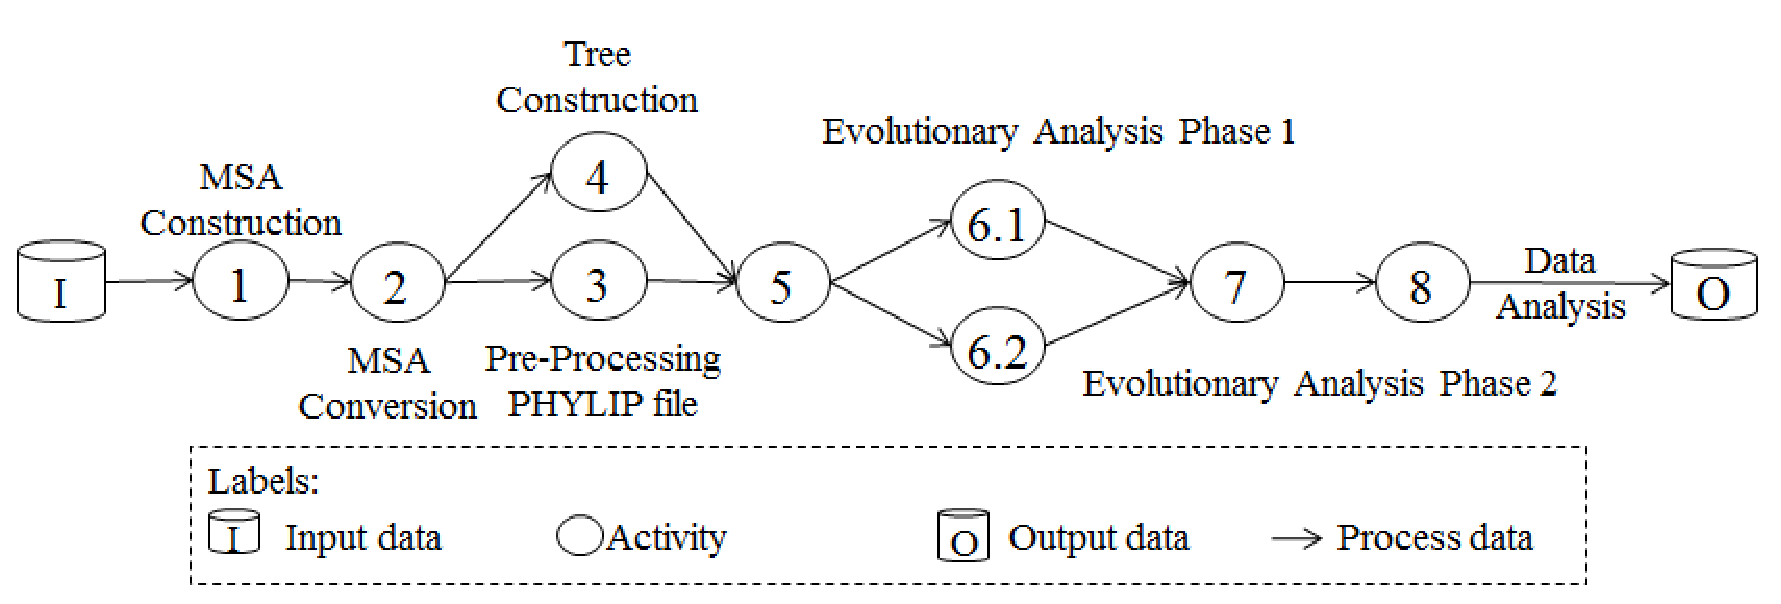
\includegraphics[width=140mm]{figures/pscievol}
\par\end{centering}
\caption{\textbf{SciEvol Scientific Workflow. }}
\label{fig:pscievol}
\end{figure*}

In this section, in order to validate the SSVP approach, we present a use case, \textit{i.e.} SciEvol with two analysis phase.
As presented in Section \ref{subsubsec:SWE}, SciEvol \cite{Ocana2012} is a SWf for molecular evolution reconstruction that aims at inferring evolutionary relationships, namely to detect positive Darwinian selection, on genome data. It has data and compute intensive activities with data constraints. These characteristics are important to evaluate our scheduling approaches. Figure \ref{fig:pscievol} shows the conceptual structure of SciEvol used for this chapter, which is composed of $9$ activities.


\section{Experimental Evaluation}
\label{sec:PVal}


\begin{table*}[htbp]
\caption{\textbf{Parameters of different types of VMs. } Type represents the type of VMs. vCPUs represents the number of virtual CPUs in a VM. RAM represents the size of memory in a VM. Disk represents the size of the hard disk in a VM. CC represents the computing capacity of VMs. MC represents Monetary Cost.} 
\label{tab:pVMP}
\begin{centering}
\captionsetup{justification=centering}
\begin{tabular}{|c|c|c|c|c|c|c|c|}
\hline 
Type & vCPUs & RAM & Disk & CC & MC \tabularnewline
\hline 
A1 & 1 & 1.75 & 70 & 9.6 & 0.0604 \tabularnewline
A2 & 2 & 3.5 & 135 & 19.2 & 0.1208\tabularnewline
A3 & 4 & 7 & 285 & 38.4 & 0.2416 \tabularnewline
A4 & 8 & 14 & 605 & 76.8 & 0.4832 \tabularnewline
\hline 
\end{tabular}
\par\end{centering} 
\end{table*}

In this section, we present an experimental evaluation of the SSVP algorithm by comparing it with GraspCC. 
The experiments show the advantages of SSVP over GraspCC in two aspects. The first aspect is that SSVP can estimate cost more accurately based on our proposed cost model than GraspCC. The second aspect is that the provisioning plans generated by SSVP incur less cost than that generated by GraspCC. 
All experiments are based on the execution of the SciEvol SWf in the Japan East region of Microsoft Azure cloud.
During the experiments, the life circle of VM is composed of creation, start, configuration, stop and deletion. The creation, start, stop and deletion of a VM is managed by using Azure CLI. The configuration of VM is realized by Linux \textit{SSH} command.
In the experiments, the execution of SWfs is performed by Chiron \cite{Ogasawara2013}. 
The goal is to show that SSVP is suitable to dynamic provisioning of VMs by making a good trade-off among different objectives for the execution of SWfs. Microsoft Azure provides $5$ tiers of VM, which are basic tier, standard tier, optimized compute, performance optimized compute and compute intensive. Each tier of VM contains several types of VMs. In one Web domain, users can provision different types of VMs at the same tier. In our experiments, we consider $4$ types, namely $A1$, $A2$, $A3$, and $A4$, in the standard tier. The features of the VM types are summarized in Table \ref{tab:pVMP}. In Azure, the time quantum is one minute. In addition, the average time to provision a VM is estimated as $2.9$ minutes. Each VM uses Linux Ubuntu $12.04$ ($64$-bit), and is configured with the necessary software for SciEvol. All VMs are configured to be accessed using Secure Shell (SSH).

\begin{table}[htbp]
\caption{\textbf{Workload Estimation. }} 
\label{app:pWE}
\begin{centering}
\captionsetup{justification=centering}
\begin{tabular}{|c|c|c|c|}
\hline 
\multirow{ 3}{*}{Activity} & \multicolumn{3}{|c|}{Number of Fasta Files} \\
\cline{2-4}
& $100$ & $500$ & $1000$ \\
\cline{2-4}
& \multicolumn{3}{|c|}{Estimated Workload (in GFLOP)} \tabularnewline
\hline
$1$ & $1440$ & $10416$ & $20833$ \tabularnewline
$2$ & $384$ & $2778$ & $5556$ \tabularnewline
$3$ & $576$ & $4167$ & $8333$ \tabularnewline
$4$ & $1440$ & $10416$ & $20833$ \tabularnewline
$6.1$ & $5760$ & $41667$ & $83334$ \tabularnewline
$6.2$ & $10560$ & $76389$ & $152778$ \tabularnewline
$6.3$ & $49920$ & $361111$ & $722222$ \tabularnewline
$6.4$ & $59520$ & $430556$ & $861111$ \tabularnewline
$6.5$ & $75840$ & $548611$ & $1097222$ \tabularnewline
$6.6$ & $202560$ & $1465278$ & $2930556$ \tabularnewline
$8$ & $6720$ & $48611$ & $97222$ \tabularnewline
\hline 
\end{tabular}
\par\end{centering} 
\end{table}

In the experiments, we use $100$, $500$, $1000$ fasta files generated from the data stored in a genome database \cite{Oma}\cite{OmaGroup}. The programs used are: mafft (version $7.221$) for Activity $1$, ReadSeq $2.1.26$ for Activity $2$, raxmhpc ($7.2.8$ alpha) for Activity $4$, pamlX$1.3.1$ for Activities $6.1 - 6.2$, in-house script for Activity $3$ and Activity $8$, and Activity $5$ and Activity $7$ exploit a PostgreSQL database management system to process data. The percentage of the workload, \textit{i.e.} $\alpha$ in Formula \ref{eq:peq9}, that can be parallelized is $96.43\%$. In addition, the input data of the SWf is stored at a data server of Site $3$, which is accessible to all the sites in the cloud using \textit{SCP} command (a Linux command). The estimated workload (in GFLOP) of each activity of SciEvol SWf for different numbers of input fasta files is shown in Table \ref{app:pWE}. 

In the tables and figures, the unit of time is minute, the unit of monetary cost is Euro, the unit of RAM and Disk is Gigabytes, the unit of data is MegaByte (MB), the computing capacity of VMs is GigaFLOPS (GFLOPS) and the unit of workload is GigaFLOP (GFLOP). $\omega_t$ represents the weight of time cost. $A1$, $A2$, $A3$ and $A4$ represent the types of VMs in Azure. [Type of VM] * [number] represents provisioning [number] of VMs of [Type of VM] type, \textit{e.g.} A1 * 1 represents provisioning one VM of A1 type. WE represents West Europe; JW Japan West and JE Japan East. The cost corresponds to the price in Euro of Azure on July 27, 2015.

\begin{table*}[htbp]
\caption{\textbf{VM Provisioning Results. }} 
\label{tab:pVMD}
\begin{centering}
\captionsetup{justification=centering}
\begin{tabular}{|c|c|c|c|c|c|c|c|}
\hline
\multicolumn{2}{{|c|}}{Algorithm} & \multicolumn{3}{{|c|}}{SSVP}  & \multicolumn{3}{|c|}{GraspCC} \tabularnewline
\hline 
\multicolumn{2}{{|c|}}{$\omega_t$} & 0.1 & 0.5 & 0.9 & 0.1 & 0.5 & 0.9\tabularnewline
\hline 
\multicolumn{2}{{|c|}}{Provisioning Plan} & $A3 * 1$ & $A4 * 1$ & $A4 * 3$ & $A1 * 6$ & \multicolumn{2}{|c|}{$A2 * 3$} \tabularnewline
\hline 
\multirow{ 3}{*}{Estimated} & Execution Time& 95 & 55 & 34 & \multicolumn{3}{|c|}{60}\tabularnewline
& Monetary Cost & 0.38 & 0.44 & 0.75 & \multicolumn{3}{|c|}{0.36}\tabularnewline
\cline{2-8}
& Cost  & 1.3094 & 1.1981 & 0.7631 & 1.1882 & 1.104 & 1.0208\tabularnewline
\hline
\multirow{ 3}{*}{Real} & Execution Time& 98 & 54 & 35 & 113 & \multicolumn{2}{|c|}{100}\tabularnewline
& Monetary Cost & 0.40 & 0.43 & 0.81 & 0.64 & \multicolumn{2}{|c|}{0.60}\tabularnewline
\cline{2-8}
& Cost & 1.3472 & 1.1748 & 0.7879 & 2.1181 & 1.8199 & 1.6973\tabularnewline
\hline 
\end{tabular}
\par\end{centering} 
\end{table*}

We execute the SciEvol SWf with $100$ fasta files for different weights of execution time and monetary costs. We assume that the limitation of the number of virtual CPU cores is $32$. The estimated workload of this SWf is $192,000$ GFLOP. The desired execution time is set to $60$ minutes and the maximum execution time is defined as $120$ minutes. The desired monetary cost is configured as $0.3$ Euros and the maximum monetary cost is $0.6$ Euros. The deployment plans presented in Table \ref{tab:pVMD} are respectively generated by SSVP, and GraspCC  \cite{Coutinho2014}. Table \ref{tab:pVMD} shows the result of the experiments to execute the SWf with different weights of execution time and monetary costs. The execution time, monetary cost and cost is composed of the time or the cost of VM provisioning and SWf execution. For SSVP, the difference between estimated and real execution time ranges from $1.9\%$ to $3.1\%$, the difference for monetary cost ranges from $2.0\%$ to $6.5\%$ and the difference for the cost is between $2.0\%$ to $3.2\%$. In fact, the difference between the estimated and real values also depends on the parameters configured by the users. Table \ref{tab:pVMD} shows that SSVP can make an acceptable estimation based on different weights of objectives, \textit{i.e.} time and monetary costs.

\begin{figure}[htbp]
\begin{centering}
\captionsetup{justification=centering}
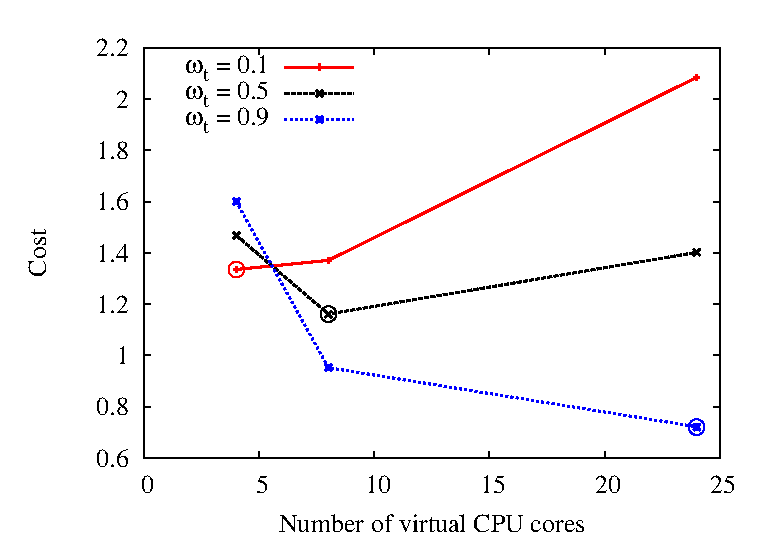
\includegraphics[width=90mm]{figures/FIG6}
\par\end{centering}
\caption{\textbf{Cost for different values of $\omega_t$ with three provisioning plans.} The circled points represent the number of virtual CPU cores corresponding to the provisioning plan generated by SSVP and the corresponding cost of the execution of SciEvol SWf.}
\label{fig:pcost}
\end{figure}

GraspCC is based on two strong assumptions. The first assumption is that the entire workload of each activity can be executed in parallel, which may not be realistic since some activities cannot be parallelized. The second one is that more VMs can reduce execution time without any bad impact on the cost, \textit{e.g.} higher monetary cost, for the whole execution of a SWf. These two assumptions lead to inaccuracies of the estimation of execution time and monetary costs. In addition, as it is only designed for the time quantum of one hour, GraspCC always generates a provisioning plan that contains the possible largest number of virtual CPUs to reduce the execution time to one time quantum, namely one hour. In Azure, since the time quantum is one minute, it is almost impossible to reduce the execution time to one time quantum, namely one minute. In order to use GraspCC in Azure, we take the time quantum of one hour for GraspCC. GraspCC does not take into consideration the cost (time and monetary costs) to provision VMs, which also brings inaccuracy to the estimated time. Moreover, GraspCC is not sensitive to different values of weight, which are $\omega_t$ and $\omega_m$. But SSVP is sensitive to different values of weight because of using the optimal number of virtual CPUs calculated based on the cost model. The final provisioning plan of GraspCC is listed in Table \ref{tab:pVMD}.
GraspCC generates the same provisioning plan for different values of $\omega_t$ ($0.5$ and $0.9$). In addition, the difference between the estimated time and the real time is $88.3$\% ($\omega_t = 0.1$) and $66.7\%$ ($\omega_t = 0.5$ and $\omega_t = 0.9$).
However, the difference corresponding to the cost model of SSVP is under $3.1\%$. Finally, compared with SSVP, the corresponding real cost of the GrapsCC algorithm is $57.2$\% ($\omega_t = 0.1$), $54.9$\% ($\omega_t = 0.5 $) and $115.4$\% ($\omega_t = 0.9$) bigger.


\begin{table}[htbp]
\caption{\textbf{Setup Parameters. } ``Number'' represents the number of input fasta files. ``Limit'' represents the maximal number of virtual CPUs that can be instantiated in the cloud. Maximum values are twice the desired values. }
\label{tab:pVMD510}
\begin{centering}
\captionsetup{justification=centering}
\begin{tabular}{|c|c|c|c|c|}
\hline
\multicolumn{2}{{|c|}}{Number} & $500$  & $1000$ \tabularnewline
\hline 
\multirow{2}{*}{Desired} & Execution Time & $60$   & $60$ \tabularnewline
 & Monetary Cost & $2$   & $6$ \tabularnewline
\hline 
\multirow{2}{*}{Maximum} & Execution Time & $120$   & $120$ \tabularnewline
 & Monetary Cost & $4$ & $12$ \tabularnewline
\hline 
\multicolumn{2}{{|c|}}{Limit} & $64$ & $128$ \tabularnewline
\multicolumn{2}{{|c|}}{Estimated Workload} & $1,401,600$ & $2,803,200$ \tabularnewline
\hline
\end{tabular}
\par\end{centering}
\end{table}

Figure \ref{fig:pcost} shows the cost for different provisioning plans and different weights of execution time and monetary costs. According to the provisioning plan generated by SSVP, $4$, $8$ and $24$ virtual CPU cores are instantiated when $\omega_t$ is $0.1$, $0.5$ and $0.9$. The corresponding cost is the minimum value in each polyline. The three polylines show that  SSVP can generate a good VM provisioning plan, which reduces the cost based on the cost model. The differences between the highest cost and the cost of corresponding good provisioning plans are: $56.1$\% ($\omega_t = 0.1$), $26.4$\% ($\omega_t = 0.5$) and $122.1$\% ($\omega_t = 0.9$). 

\begin{table*}[htbp]
\caption{\textbf{SSVP VM Provisioning Results. } ``Number'' represents the number of input fasta files. The provisioning plan represents the plan generated by the corresponding algorithms. "ET" represents execution time and "MC" represents monetary cost.}
\label{tab:pVMD511}
\begin{centering}
\captionsetup{justification=centering}
\begin{tabular}{|c|c|c|c|c|c|c|c|}
\hline
\multicolumn{2}{{|c|}}{Number} & \multicolumn{3}{{|c|}}{$500$}  & \multicolumn{3}{|c|}{$1000$} \tabularnewline
\hline 
\multicolumn{2}{{|c|}}{$\omega_t$} & 0.1 & 0.5 & 0.9 & 0.1 & 0.5 & 0.9\tabularnewline
\hline
\multicolumn{2}{{|c|}}{Provisioning Plan} & $A2 * 1, A4 * 1$ & $A4 * 3$ & $A4 * 7$ & $A4 * 2$ & $A4 * 6$ & $A4 * 11$ \tabularnewline
\hline
\multirow{3}{*}{Estimated} & ET & $328$ & $194$ & $150$ & $473$ & $290$ & $260$ \tabularnewline
& MC & $3.29$ & $4.60$ & $7.93$ & $7.59$ & $13.62$ & $21.70$ \tabularnewline
& Cost & $2.0263$ & $2.7640$ & $2.6419$ & $1.9271$ & $3.5462$ & $4.2602$ \tabularnewline
\hline
\multirow{3}{*}{Real} & ET & $299$ & $177$ & $136$ & $424$ & $294$ & $244$ \tabularnewline
& MC & $2.99$ & $4.42$ & $8.34$ & $6.90$ & $14.71$ & $23.21$ \tabularnewline
& Cost & $1.8438$ & $2.5800$ & $2.4572$ & $1.7417$ & $3.6758$ & $4.0468$ \tabularnewline
\hline
\end{tabular}
\par\end{centering}
\end{table*}

\begin{table*}[htbp]
\caption{\textbf{GraspCC VM Provisioning Results. } ``Number'' represents the number of input fasta files. The provisioning plan represents the plan generated by the corresponding algorithms.}
\label{tab:pVMD512}
\begin{centering}
\captionsetup{justification=centering}
\begin{tabular}{|c|c|c|c|c|c|c|c|}
\hline
\multicolumn{2}{{|c|}}{Number} & \multicolumn{3}{{|c|}}{$500$}  & \multicolumn{3}{|c|}{$1000$} \tabularnewline
\hline
\multicolumn{2}{{|c|}}{Provisioning Plan} & \multicolumn{3}{{|c|}}{$A1 * 1$, $A3 * 10$} & \multicolumn{3}{{|c|}}{$A2 * 1$, $A4 * 10$}  \tabularnewline
\hline
\multirow{3}{*}{Estimated} & Execution Time & \multicolumn{3}{{|c|}}{$60$} & \multicolumn{3}{{|c|}}{$60$} \tabularnewline
& Monetary Cost & \multicolumn{3}{{|c|}}{$2.48$} & \multicolumn{3}{{|c|}}{$4.95$} \tabularnewline
\cline{3-8}
& Cost & 1.2144 & 1.1191 & 1.0238 & 0.8429 & 0.9127 & 0.9825 \tabularnewline
\hline
\multirow{3}{*}{Real} & Execution Time & \multicolumn{3}{{|c|}}{$166$} & \multicolumn{3}{{|c|}}{$257$} \tabularnewline
& Monetary Cost & \multicolumn{3}{{|c|}}{$6.19$} & \multicolumn{3}{{|c|}}{$22.43$} \tabularnewline
\cline{3-8}
& Cost & 3.06 & 2.93 & 2.80 & 3.79 & 4.01 & 4.23 \tabularnewline
\hline
\end{tabular}
\par\end{centering}
\end{table*}

We also execute SciEvol with $500$ and $1000$ fasta files. The setup parameters  are listed in Table \ref{tab:pVMD510} and the results are shown in Tables \ref{tab:pVMD511} and \ref{tab:pVMD512}. Since it needs bigger computing capacity to process more input fasta files, we increase the limitation of the number of virtual CPUs, \textit{i.e.} 64 virtual CPUs for $500$ fasta files and $128$ virtual CPUs for $1000$ fasta files. From the tables, we can see that as the estimated workload and desired monetary cost of the SWf grow, more virtual CPUs are planned to be deployed in the cloud.
SSVP generates different provisioning plans for each weight of time cost. However, for the same number of input fasta files, GraspCC generates the same provisioning plan for different weights of time cost, namely $A1 * 1$, $A3 * 10$ for 500 fasta files and $A2 * 1$, $A4 * 10$ for 1000 fasta files. The execution time corresponding to both SSVP and GraspCC, exceeds the maximum execution time. However, SSVP has some important advantages, \textit{e.g.} precise estimation of execution time and smaller corresponding cost.

\begin{figure}[htbp]
\begin{centering}
\captionsetup{justification=centering}
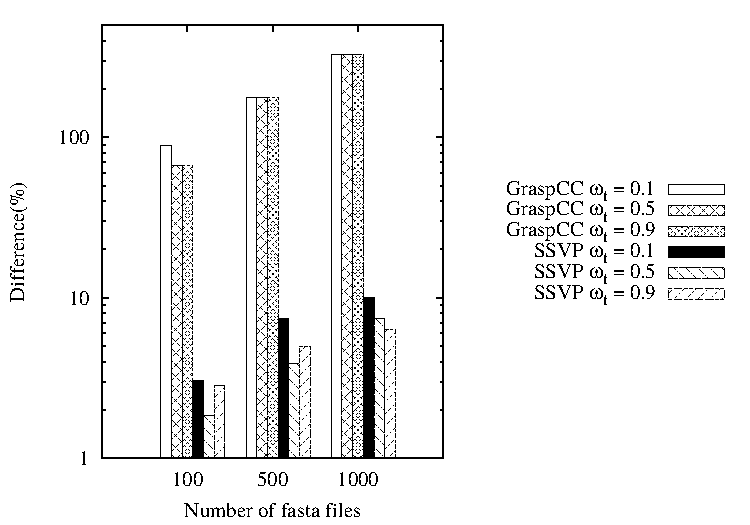
\includegraphics[width=90mm]{figures/FIG7}
\par\end{centering}
\caption{\textbf{Difference between estimated time and real time. }}
\label{fig:pDIFF}
\end{figure}

The difference between estimated time and real time is calculated based on Formula \ref{eq:peq19}. As shown in Figure \ref{fig:pDIFF}, the difference between estimated execution time and real execution time corresponding to GraspCC is much higher than that corresponding to the cost model of SSVP, which ranges between $66.7\%$ and $328.3\%$. This result reveals that our cost model can be up to $76.7\%$ more precise than that of GraspCC. As the number of fasta files increases, the difference goes up, \textit{i.e.} it is more difficult to estimate the time. However, the difference corresponding to the cost model of SSVP is always under $11\%$. 

\begin{equation}\label{eq:peq19}
Difference = \frac{EstimatedTime - RealTime}{RealTime} * 100 \%
\end{equation}

The cost corresponding to different numbers of fasta files is shown in Figure \ref{fig:pcomparisionD}. It can be seen from Figure \ref{fig:pc1}, Figure \ref{fig:pc5} and Figure \ref{fig:pc10} that the cost corresponding to GraspCC is always higher than that corresponding to SSVP with different amounts of input data because SSVP is based on a more accurate cost model and is designed for the quantum of one minute. Based on Formula \ref{eq:peq20}, compared with GraspCC, the cost corresponding to SSVP is up to $53.6\%$ smaller. The cost for GraspCC is a line in Figures \ref{fig:pc5} and \ref{fig:pc10}, since GraspCC is not sensitive to the weights of time cost and it generates the same VM provisioning plans, the cost of which is a line. However, since SSVP is sensitive to different values of the weights of execution time, it can reduce the cost at large.
\begin{equation}\label{eq:peq20}
Difference = \frac{Cost(GraspCC) - Cost(SSVP)}{Cost(SSVP)} * 100 \%
\end{equation}


\begin{figure*}[htbp]
\begin{centering}
		\subfigure[\textbf{Cost for 100 fasta files.}]{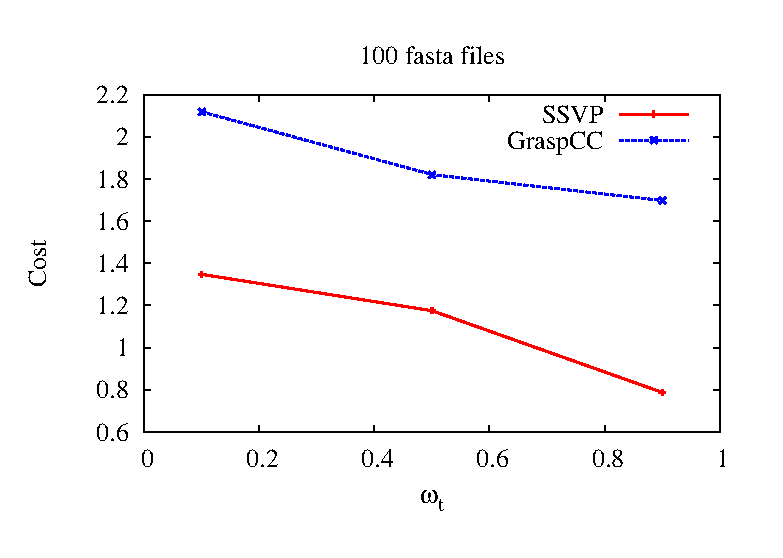
\includegraphics[width=59mm]{figures/FIG8_1} \label{fig:pc1}}
		\subfigure[\textbf{Cost for 500 fasta files.} ]{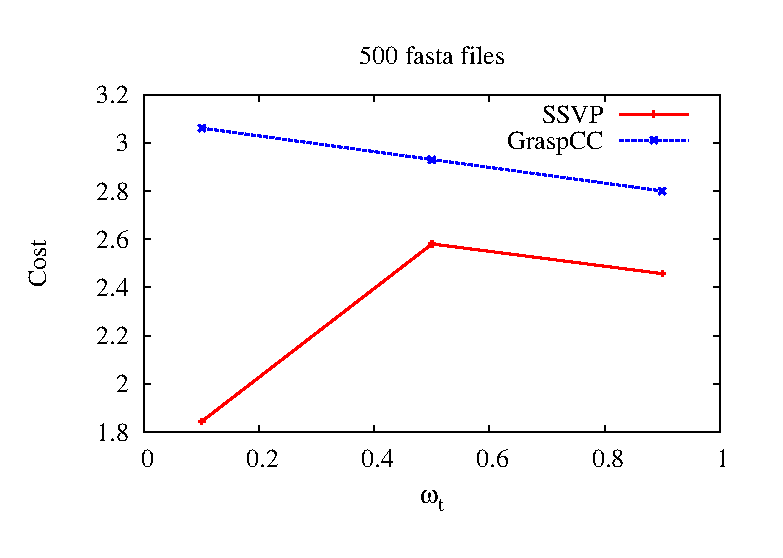
\includegraphics[width=59mm]{figures/FIG8_2} \label{fig:pc5}}
		\subfigure[\textbf{Cost for 1000 fasta files.}]{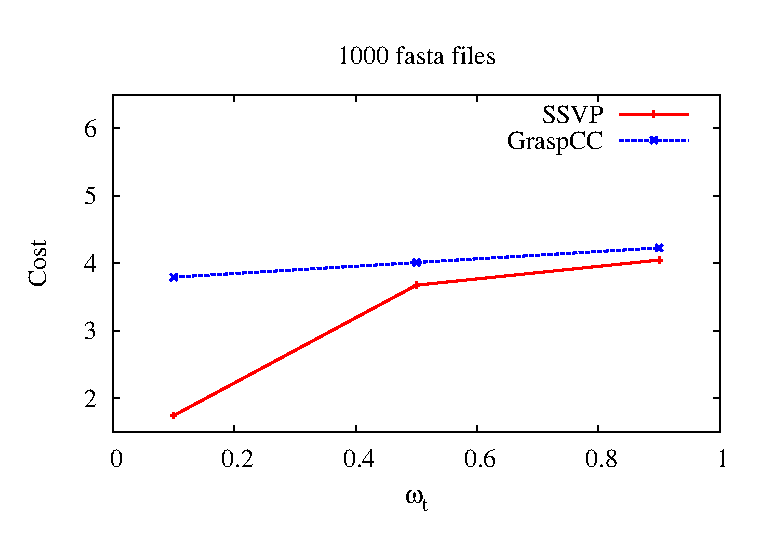
\includegraphics[width=59mm]{figures/FIG8_3} \label{fig:pc10}}
\caption{\textbf{Cost for different numbers of fasta files.}}\label{fig:pcomparisionD}
\end{centering}
\end{figure*}
From the experimental results, we can get the conclusion that SSVP can generate better VM provisioning plans than GraspCC because of accurate cost estimation of the cost model. 

\section{Conclusion}
\label{sec:PCon}

In this chapter, we proposed a new VM provisioning approach, namely SSVP, to generate VM provisioning plans for SWf execution with multiple objectives in a single site cloud. The cost model aims at minimizing two costs: execution time and monetary costs.
We used a real SWf that is SciEvol, with real data from the bioinformatics domain as a use case. We evaluated our approaches by executing SciEvol in Microsoft Azure cloud. The results show the provisioning approach (SSVP) generates better provisioning plans for different weights of time cost to execute a SWf at a site, compared with other existing approaches, namely GraspCC. The advantage of SSVP can be up to $53.6\%$. In addition, our cost model can estimate the cost within an acceptable error limit and it is $76.7\%$ more precise than that of GraspCC.